%% ============================================================
%%  Chapter 4 — Results
%%  Princeton CBE Senior Thesis — RNA–ASO Modeling Pipeline
%% ============================================================

\chapter{Results}
\label{chap:results}

%% --------------------------------------------------------
\section{Overview}
\label{sec:results-overview}
%% --------------------------------------------------------

While sequence complementarity can give some indication of where on an RNA 
hairpin an antisense oligonucleotide will bind, it does not always provide reliable information as 
to whether these sequences are available for interaction with an antisense oligonucleotide. A site 
may appear to be complementary but it could be base paired and therefore unavailable for interaction 
with the antisense oligonucleotide. The site may also exist in three dimensional space that prevents it 
from being able to interact with the antisense oligonucleotide or it could be exposed for such short 
periods of time that there is no possibility of interaction.

The remainder of this Chapter provides a step-by-step approach to addressing this issue. Using the 
RNA structure derived from PDB ID: 1YMO we will analyze each site within our target RNA to determine 
whether they have potential as targets for antisense oligonucleotides. We begin by analyzing RNA 
structural dynamics within the loop/core region. Is the loop/core region of the RNA dynamic? Does 
the degree of structural dynamics depend upon the presence of ASOs and/or their design?

Next we examine two dimensional accessibility. Which residues within our target RNA are likely to 
be unpaired in the average population of conformations. Finally we perform three-dimensional 
accessibility by determining solvent accessible surface area (SASA) for all residues.

Our last task is to use computational methods to simulate binding events between ASOs and our target 
RNA. This simulation allows us to evaluate the feasibility of using a particular ASO at a particular 
location based upon a center of mass distance. In many cases, when using this method, we obtain a 
ranking of feasible ASO locations that is different than that obtained using sequence complementarity 
alone.


%% --------------------------------------------------------
\section{RNA structural dynamics are sensitive to ASO loading and design}
\label{sec:results-dynamics}
%% --------------------------------------------------------

%% NOTE: confirm \ref{app:rmsd-scaling} exists in your source before compiling
As context, mean RMSD scales monotonically with RNA sequence length across the
50-, 100-, and 200-nucleotide systems simulated (full data in
Appendix~\ref{app:rmsd-scaling}).
The 1YMO-derived 100-nucleotide system therefore occupies an intermediate
dynamic regime between the shorter and longer constructs.
For the present pipeline, the more informative quantity is loop-core RMSF,
which isolates fluctuations in the apical loop region that defines the
primary candidate target site.

Loop-core RMSF changes across both ASO loading conditions and ASO design
perturbations (Figure~\ref{fig:rmsf-summary}), though in both cases the
shift is quantitative rather than qualitative.
Loop flexibility persists under every condition tested.

\paragraph{Effect of ASO count.}
Mean loop-core RMSF across the four loading levels does not decrease
monotonically with ASO count
(Figure~\ref{fig:rmsf-summary}A).
At 25~ASOs the mean is 29.02~\AA;
it decreases to 26.87~\AA\ at 50~ASOs, rises to 31.45~\AA\ at 100~ASOs,
and drops again to 24.64~\AA\ at 200~ASOs.
The 100-ASO condition produces the highest loop-core RMSF of any loading
level---an anomaly rather than a trend---and the overall span across all four
conditions is roughly 7~\AA.
The mechanism behind the non-monotonicity at 100~ASOs is not resolved by
these simulations and the effect should be interpreted with caution.
Varying ASO number within the tested range produces modest, non-systematic
changes in loop dynamics; the pipeline does not depend on a particular
loading level to define accessibility.

\paragraph{Effect of ASO design.}
The design comparison is more informative.
Among the ten 100-ASO variants, loop-core RMSF spans from 23.19~\AA\
(Unmodified Loop Gg$\rightarrow$Aa) to 31.45~\AA\ (Unmodified), a range of
roughly 8~\AA\ (Figure~\ref{fig:rmsf-summary}B).
The Scrambled variant (30.39~\AA) sits close to the Unmodified reference,
indicating that scrambling the sequence does not substantially alter
loop-core flexibility on its own.
Mismatch variants (U5C: 28.05~\AA; G6A: 26.44~\AA) occupy the middle of the
distribution.
The extended (12mer: 24.04~\AA; 14mer: 23.61~\AA) and all-purine
(24.71~\AA) variants cluster at the low end, alongside the loop-substituted
sequence.
Design perturbations shift loop-core RMSF appreciably across the tested
variants, with the extended, all-purine, and loop-substituted sequences
occupying the low end of the distribution.
Whether those shifts correspond to more or less favorable ASO association is
addressed in Section~\ref{sec:results-binding}.

\begin{figure}[htbp]
  \centering
  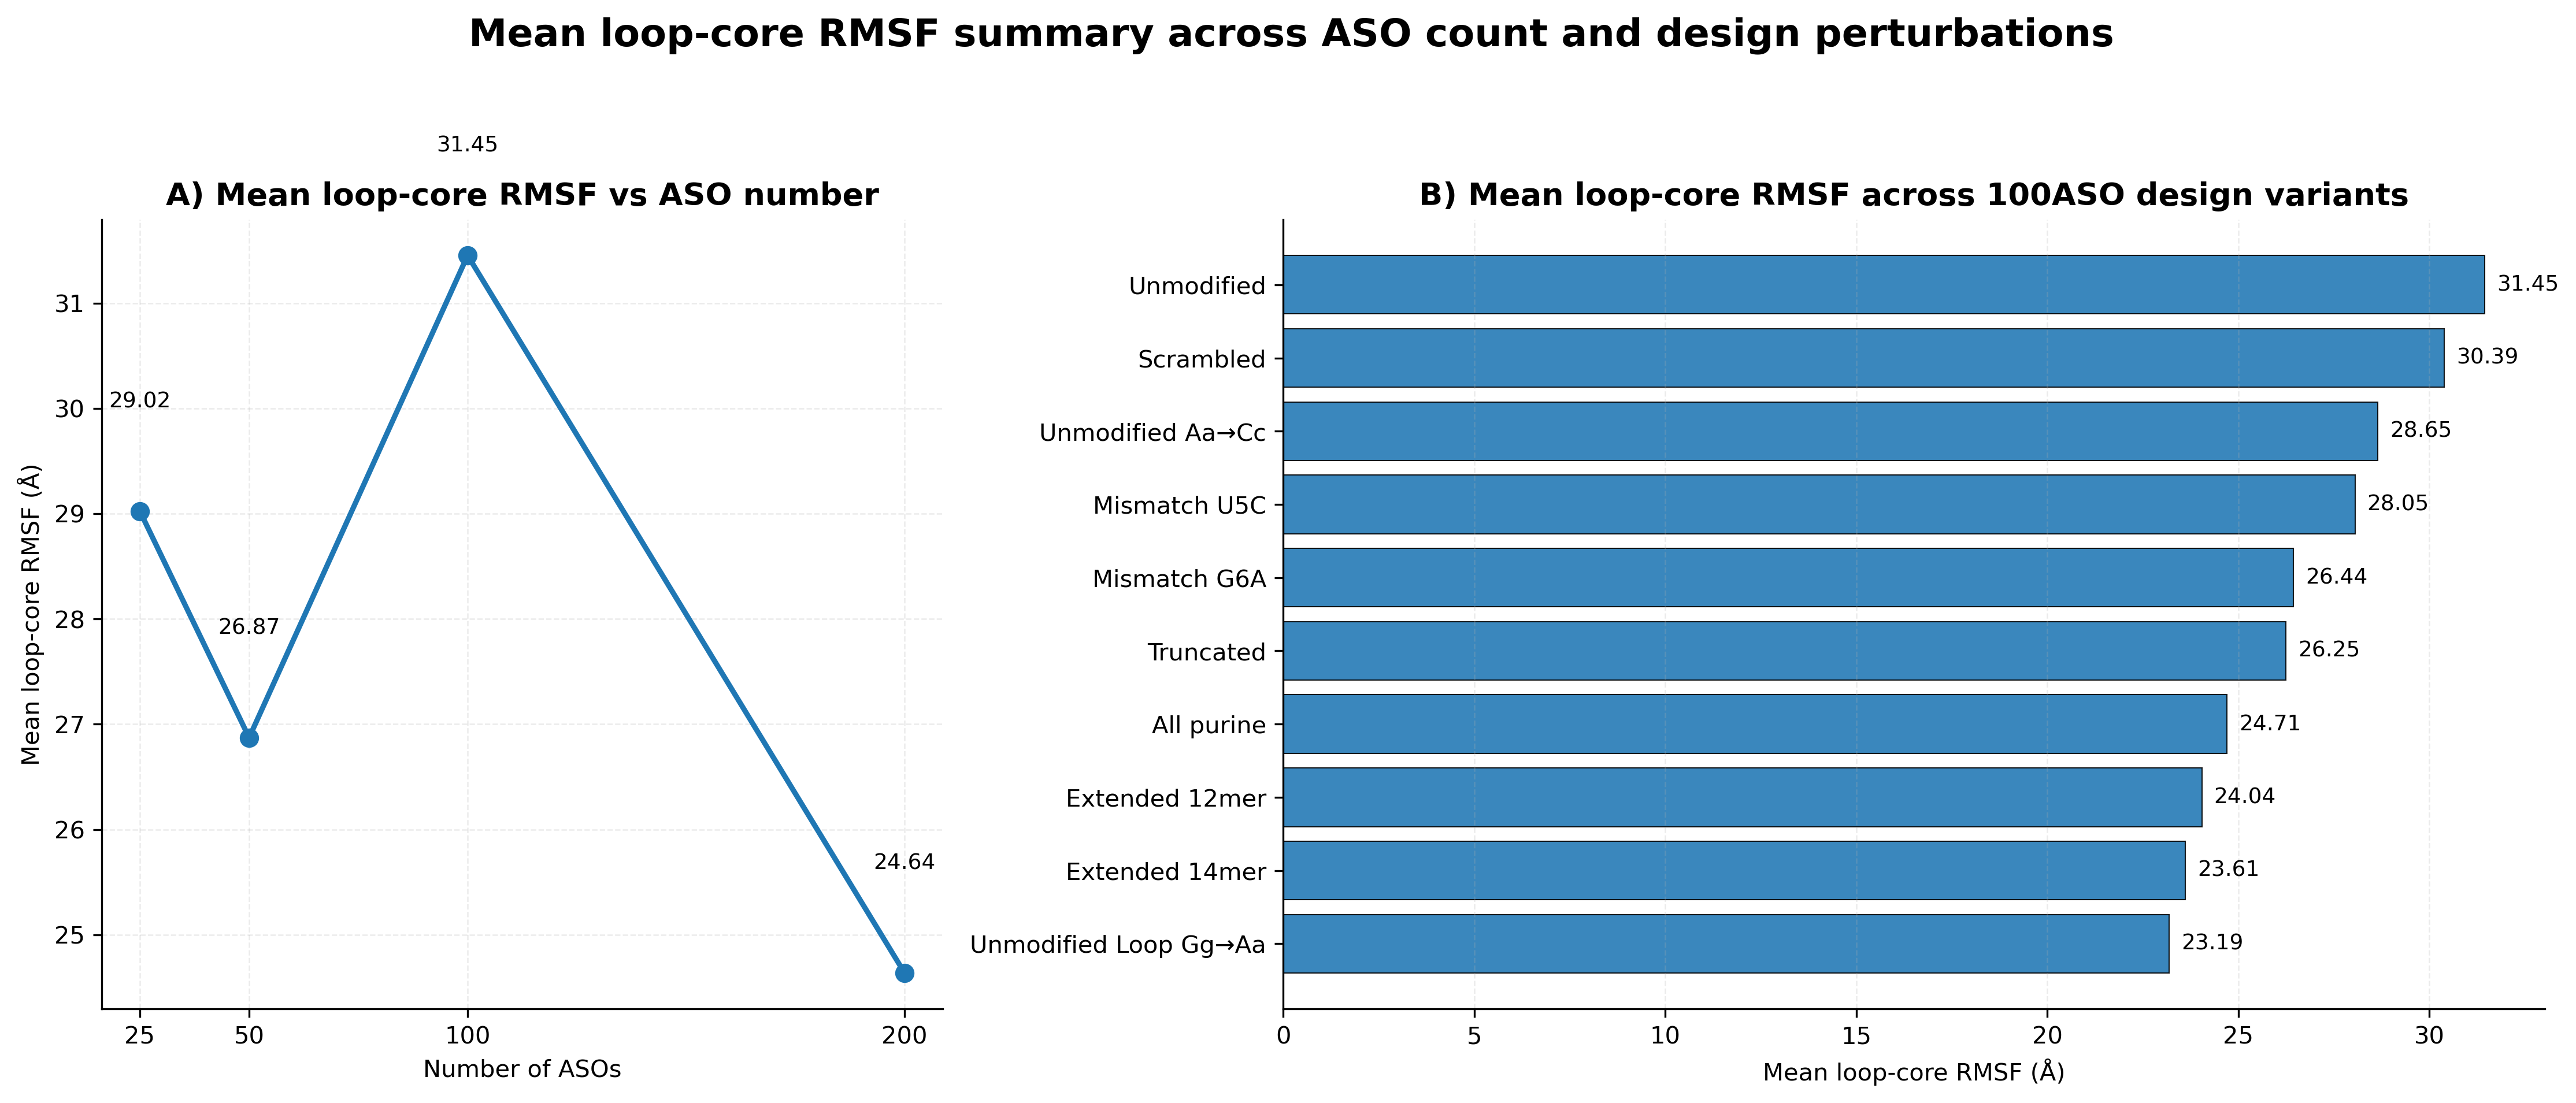
\includegraphics[width=\textwidth]{Figures/rmsf_summary.png}
  \caption{Mean loop-core RMSF across ASO conditions.
           \textbf{A:}~Mean loop-core RMSF as a function of ASO count
           (25, 50, 100, 200~ASOs).
           The relationship is non-monotonic; the 100-ASO condition yields
           the highest mean value (31.45~\AA) and the 200-ASO condition the
           lowest (24.64~\AA).
           \textbf{B:}~Mean loop-core RMSF for the ten 100-ASO design
           variants, ordered from highest to lowest.
           The Unmodified and Scrambled sequences produce the highest RMSF;
           the extended and loop-substituted variants produce the lowest.
           All values range between 23.19 and 31.45~\AA.}
  \label{fig:rmsf-summary}
\end{figure}


%% --------------------------------------------------------
\section{Secondary-structure analysis identifies the loop as the accessible region}
\label{sec:results-secondary}
%% --------------------------------------------------------

Ensemble secondary-structure calculations for the 1YMO-derived hairpin
identify the apical loop as the region of highest predicted
single-strandedness, while stem residues remain largely inaccessible due
to stable base-pairing.
A small set of loop-adjacent residues near the stem junction shows
intermediate accessibility, consistent with partial fraying in the
trajectory ensemble.
Stem residues are deprioritized on this basis; the loop region is carried
forward for three-dimensional accessibility analysis.


%% --------------------------------------------------------
\section{Three-dimensional accessibility is localized to specific residues}
\label{sec:results-sasa}
%% --------------------------------------------------------

Within the loop region, solvent accessibility is unevenly distributed
across residues.
The SASA profile of the 1YMO-derived hairpin reference structure
(Figure~\ref{fig:sasa-profile}) shows that three-dimensional exposure is
localized to a small number of positions rather than distributed uniformly
across the loop.

Residue~16 is the dominant peak within the loop, at approximately
260~\AA$^{2}$---well above the stem residue range of roughly
130--180~\AA$^{2}$.
Residue~17 is also elevated at approximately 185~\AA$^{2}$.
The remaining loop residues occupy an intermediate range
(150--175~\AA$^{2}$ for residues 13, 15, 18--20), with residue~14
dipping to approximately 118~\AA$^{2}$ despite its loop annotation,
indicating partial burial.
Outside the annotated loop, residue~30 reaches approximately 197~\AA$^{2}$,
comparable to the better-exposed loop residues and notable given its
stem-proximal position.

Loop annotation by sequence position alone overstates the number of
well-exposed target sites.
Residue~14's partial burial and residue~30's unexpectedly high exposure
would both be missed by a purely sequence-based filter.
The SASA profile narrows the accessible candidate set: the highest-priority
target region centers on residue~16 and its immediate neighbors, while
residue~30 is flagged as a non-canonical candidate warranting separate
consideration.
These priorities inform the binding simulations described in
Section~\ref{sec:results-binding}.

The SASA values reported here are computed from the 1YMO-derived reference
structure and represent a structural snapshot rather than a
trajectory-averaged quantity.

\begin{figure}[htbp]
  \centering
  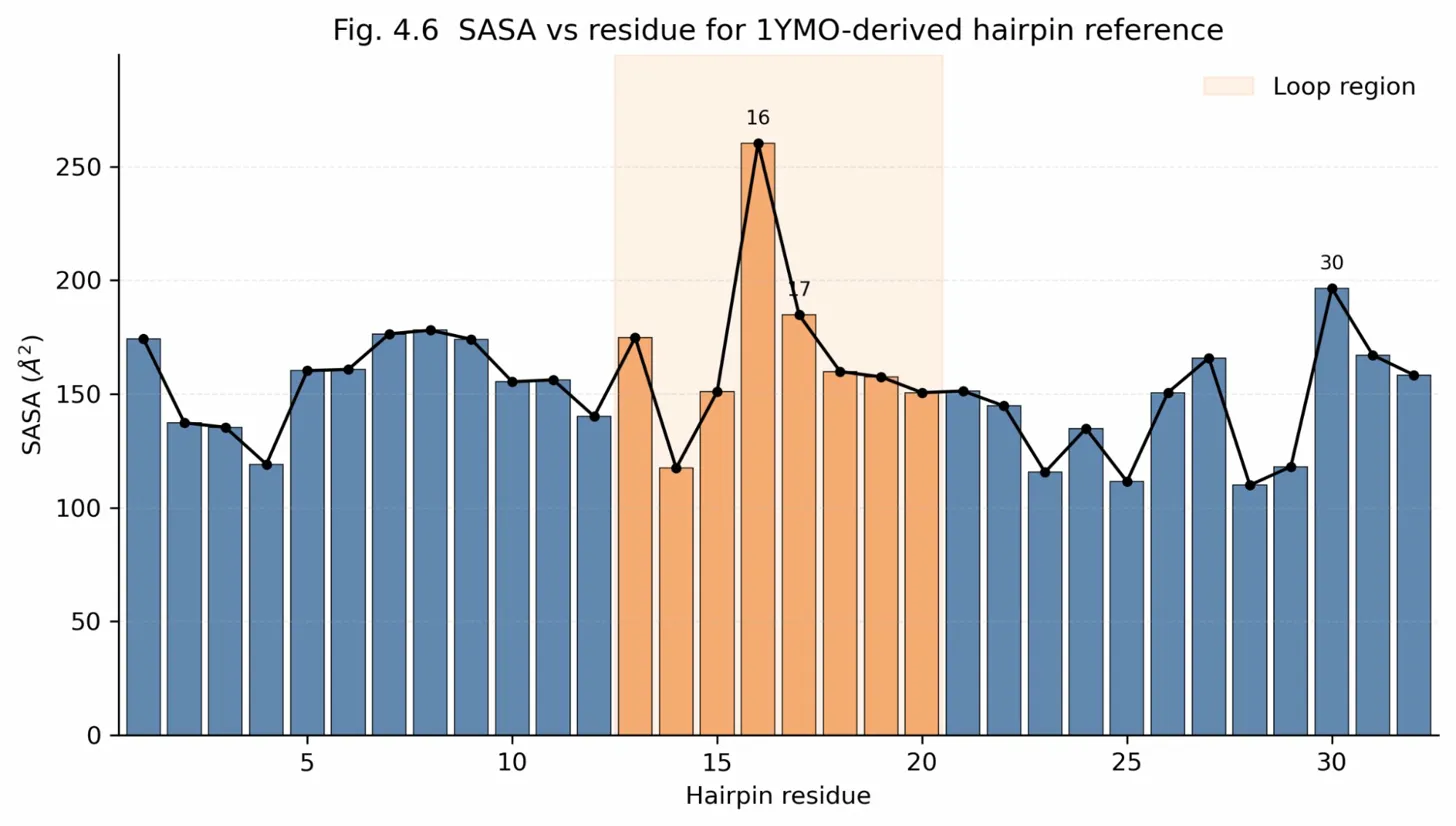
\includegraphics[width=\textwidth]{Figures/sasa_profile.png}
  \caption{SASA as a function of residue position for the 1YMO-derived
           hairpin reference structure.
           Orange bars and the orange shaded background indicate the
           annotated loop region (approximately residues 13--20).
           Blue bars indicate stem residues.
           Residue~16 is the dominant peak within the loop
           ($\approx$260~\AA$^{2}$).
           Residue~30, outside the annotated loop, also shows elevated
           exposure ($\approx$197~\AA$^{2}$).
           Residue~14 dips to $\approx$118~\AA$^{2}$ despite its loop
           position, indicating partial burial.}
  \label{fig:sasa-profile}
\end{figure}


%% --------------------------------------------------------
\section{Integrating two-dimensional and three-dimensional accessibility
         narrows candidate ASO sites}
\label{sec:results-integration}
%% --------------------------------------------------------

Taken together, the secondary-structure and SASA analyses converge on a short
list of residues that are both nominally single-stranded and solvent-exposed
in three dimensions.
Residue~16 satisfies both criteria most strongly: it is predicted to be
unpaired in the ensemble and carries the highest SASA value within the loop.
Residues~13, 15, 17, and~18 are secondary candidates, meeting both criteria at
intermediate confidence.
Residue~14 is deprioritized due to its unexpectedly low SASA despite loop
annotation.
Residue~30 is noted as a non-canonical site on SASA grounds alone, without
strong secondary-structure support for single-strandedness at that position.

This narrowed set defines the target surface against which the binding
simulations are run.


%% --------------------------------------------------------
\section{Apparent binding affinity under the COM-based metric differentiates
         candidate ASO designs}
\label{sec:results-binding}
%% --------------------------------------------------------

The final stage of the pipeline evaluates candidate ASO designs using a
center-of-mass (COM) distance-based binding metric.
The apparent dissociation constant $K_d$ derived from this metric is a
comparative quantity based on the fraction of simulation time spent at
short COM distances, normalized as described in Methods.
The numerical values---which fall in the hundreds to low thousands of mM---
are not directly comparable to experimentally measured dissociation constants
and should be read as an internal ranking rather than an absolute measure
of binding strength.
Lower apparent $K_d$ indicates more favorable association behavior
under this metric.

\paragraph{Effect of ASO count.}
Apparent $K_d$ increases with ASO number across the three loading levels
tested: 135.3~mM at 25~ASOs, 290.2~mM at 50~ASOs, and 349.7~mM at
200~ASOs (Figure~\ref{fig:kd-summary}A).
The 25-ASO condition shows lower apparent $K_d$ than the higher-count
conditions under this metric, though the difference---roughly 2.6-fold
across a factor of eight in ASO number---is modest relative to the
design-level differences described below.

\paragraph{Effect of ASO design.}
Among the ten 100-ASO design variants, apparent $K_d$ spans nearly a
tenfold range (Figure~\ref{fig:kd-summary}B).
At the less favorable end, the Extended 14mer shows 2494.2~mM,
the Extended 12mer 1152.1~mM, and Mismatch U5C 948.4~mM.
At the more favorable end, the Truncated variant shows 243.0~mM,
Unmodified Aa$\rightarrow$Cc 321.6~mM, and Unmodified Loop
Gg$\rightarrow$Aa 355.3~mM.
The Scrambled variant (740.5~mM) shows higher apparent $K_d$ than the
Unmodified reference under this metric, which is consistent with the
expectation that disrupting complementarity weakens apparent association
behavior in this framework.
The All-purine (558.9~mM) and Mismatch G6A (534.6~mM) variants occupy
intermediate positions.

The most striking pattern is the poor apparent performance of the extended
variants.
Both the 12mer and 14mer extensions produce the lowest loop-core RMSF in the
RMSF analysis yet show the highest apparent $K_d$ values here---a discordance
that is not resolved by the present simulations and is discussed further in
Chapter~\ref{chap:discussion}.
The claim here is descriptive: under the COM-based metric, longer ASO
designs are less favorable than shorter ones, even when they more
substantially suppress loop dynamics.

Design perturbations shift apparent $K_d$ across a wider range than ASO
count alone, and neither RMSF nor accessibility analysis alone would have
produced this rank ordering.

\begin{figure}[htbp]
  \centering
  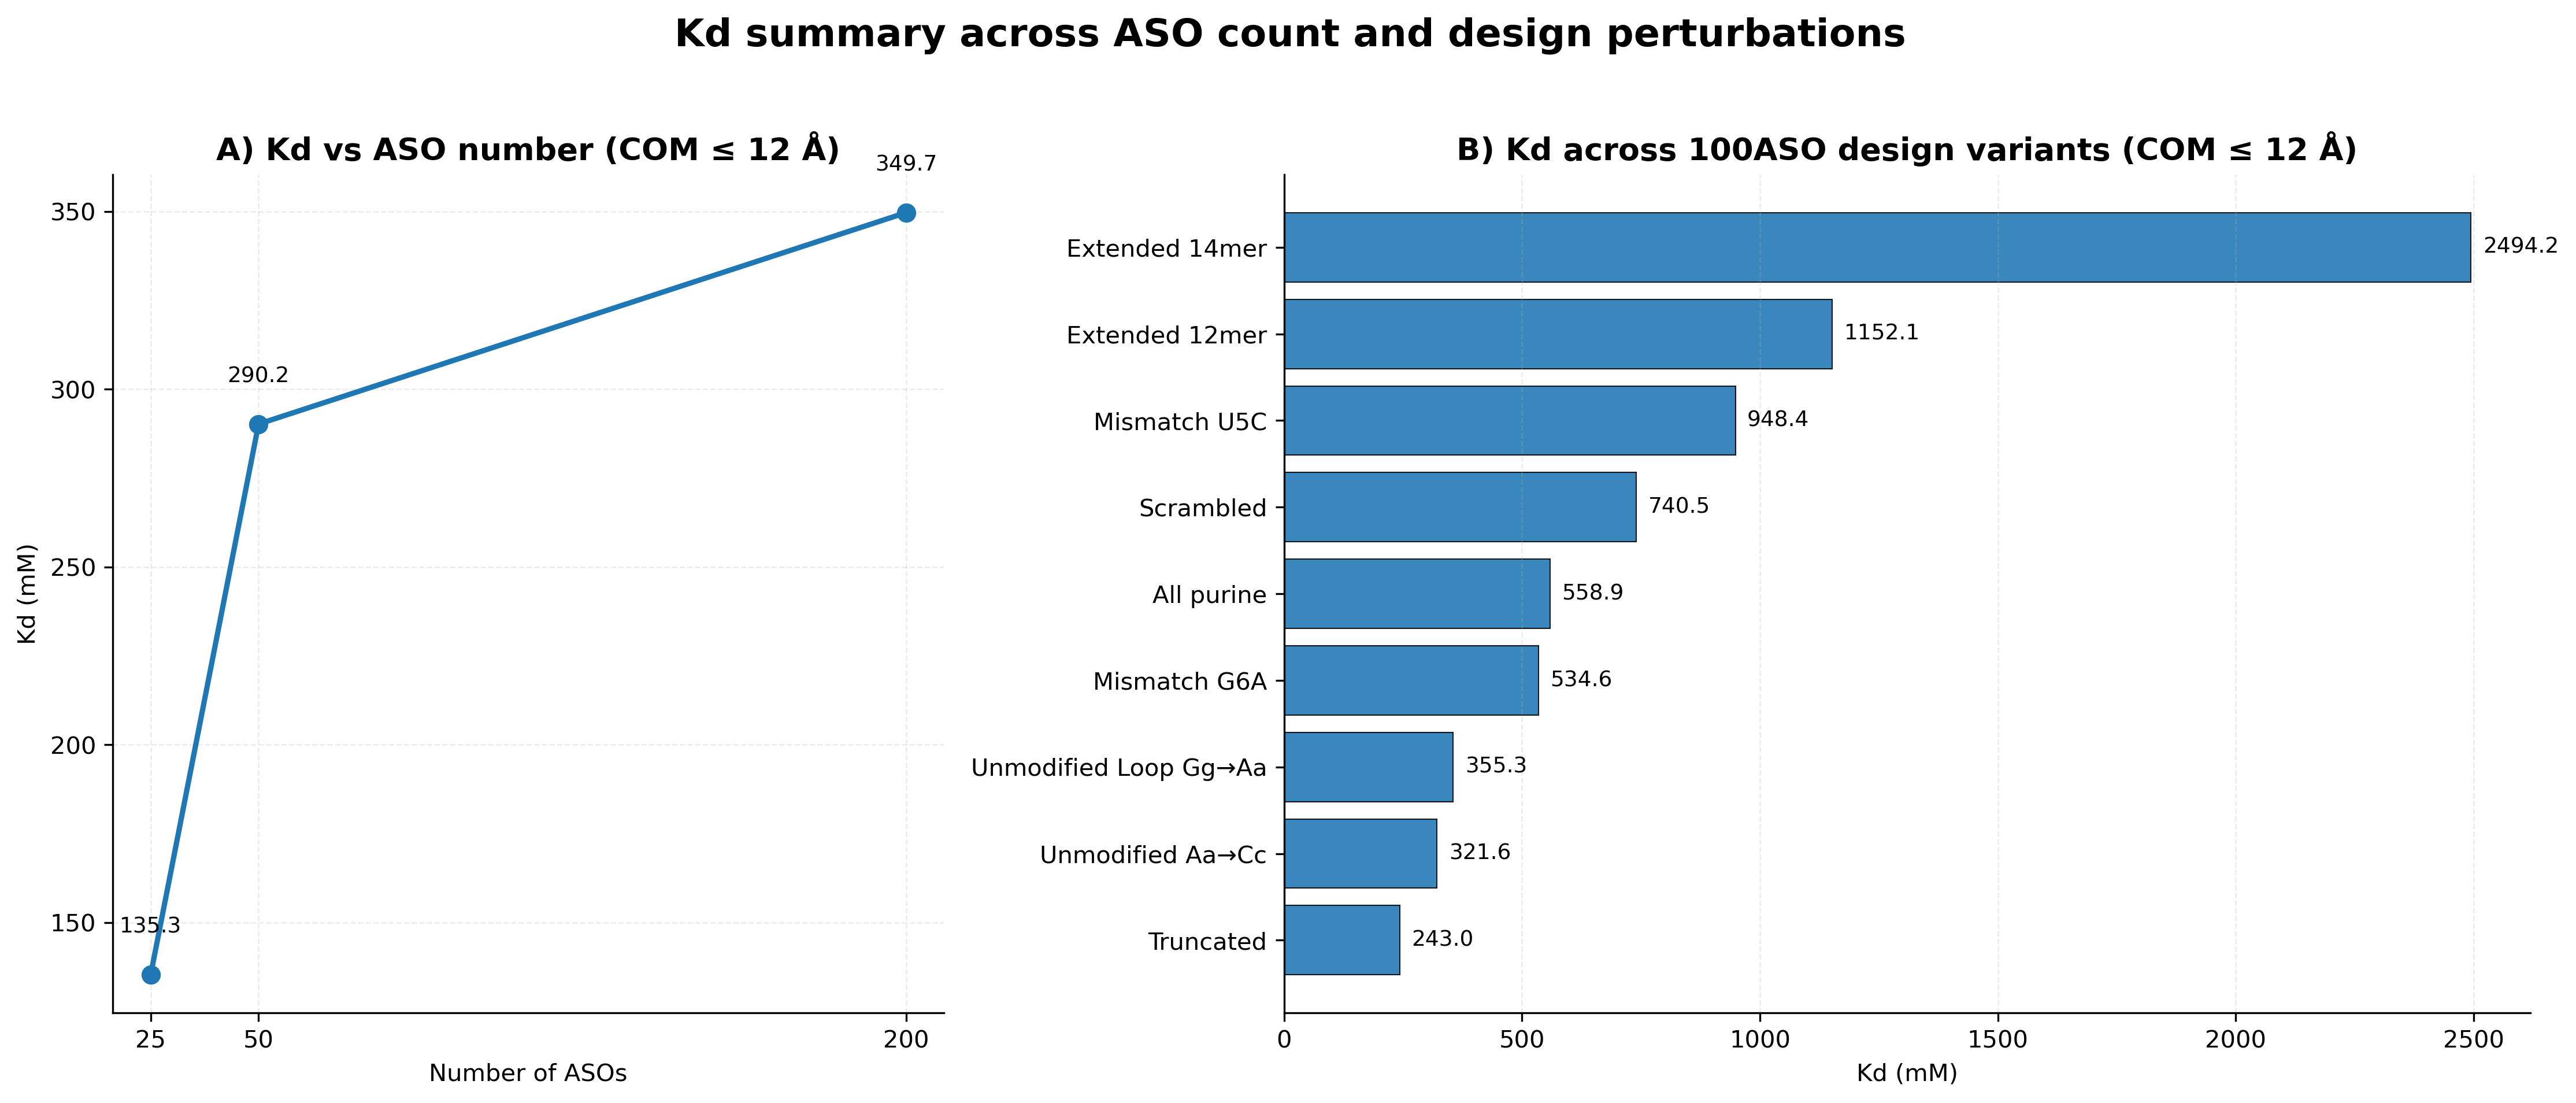
\includegraphics[width=\textwidth]{Figures/kd_summary.png}
  \caption{Apparent $K_d$ under the COM-based binding metric.
           All values are in mM and should be interpreted as a comparative
           internal ranking; they are not equivalent to experimentally
           measured dissociation constants.
           Lower apparent $K_d$ indicates more favorable association
           behavior under this metric.
           \textbf{A:}~Apparent $K_d$ as a function of ASO count (25, 50,
           200~ASOs): 135.3, 290.2, and 349.7~mM respectively.
           \textbf{B:}~Apparent $K_d$ for the ten 100-ASO design variants.
           The Extended 14mer (2494.2~mM) and Extended 12mer (1152.1~mM)
           are least favorable under this metric; the Truncated (243.0~mM)
           and Unmodified Aa$\rightarrow$Cc (321.6~mM) variants are
           most favorable.}
  \label{fig:kd-summary}
\end{figure}


%% --------------------------------------------------------
\section{Chapter synthesis}
\label{sec:results-synthesis}
%% --------------------------------------------------------

The four stages of the pipeline each contribute information that the others
cannot provide.
RMSF analysis shows that the loop-core remains dynamic across all tested
conditions, which justifies treating accessibility as an ensemble property
rather than reading off a single structure.
Secondary-structure analysis eliminates stem residues from consideration
and flags a subset of loop positions with intermediate accessibility.
SASA analysis shows that even within the loop, exposure is uneven---
residue~16 stands out clearly, and residue~14 is less exposed than its
position would suggest.
The binding simulations then produce a ranking that neither the RMSF data
nor the accessibility data anticipates: extended variants that reduce loop
fluctuation are less favorable under the COM-based metric, not more.

Two results merit acknowledgment before the Discussion.
The non-monotonic RMSF behavior at 100~ASOs does not fit a simple crowding
or stabilization narrative, and no explanation is advanced here.
The discordance between loop-dynamic suppression and apparent binding
affinity for the extended variants is the most substantively unexpected
finding in the chapter; resolving whether it reflects a real binding
penalty or a metric artifact is a central question for
Chapter~\ref{chap:discussion}.
%% NOTE: confirm \ref{chap:discussion} exists in your source before compiling

A complementarity-only selection criterion would have ranked the extended
variants highly, while the COM-based analysis ranks them last.
That reordering is the clearest empirical justification for the full
pipeline: sequence matching alone would have favored designs that the
integrated accessibility and binding analysis ultimately deprioritizes.